\documentclass[9pt,twoside,lineno]{pnas-new}
% Use the lineno option to display guide line numbers if required.

\templatetype{pnassupportinginfo}

% Math
\def\P{\mathbb{P}}
\def\cor{\mathrm{cor}}
\def\Quantile{\mathrm{Quantile}}
\def\logit{\mathrm{logit}}
\def\dist{\mathrm{dist}}
\def\WIS{\mathrm{WIS}}
\def\AUC{\mathrm{AUC}}
\newcommand{\indicator}[1]{\mathbf{1}\left(#1\right)}

% Figures and tables
\usepackage{xurl}
\usepackage{microtype}
\usepackage{booktabs}
\usepackage{caption}
\usepackage{subcaption}
\usepackage{xcolor}
\newcommand{\attn}[1]{\textcolor{red}{[ATTN: #1]}}

\makeatletter 
\renewcommand\@biblabel[1]{#1} 
\makeatother

% indicators
\newcommand{\chngcli}{CHNG-CLI}
\newcommand{\chngcov}{CHNG-COVID}
\newcommand{\dv}{DV-CLI}
\newcommand{\ar}{AR}
\newcommand{\fb}{CTIS-CLI-in-community}
\newcommand{\gs}{Google-AA}


\providecommand{\tightlist}{%
  \setlength{\itemsep}{0pt}\setlength{\parskip}{0pt}}


\title{Can Auxiliary Indicators Improve COVID-19 Forecasting and Hotspot  
  Prediction?} 

\author{Daniel J.\ McDonald, Jacob Bien, Alden Green, Addison Hu, Nat DeFries, Sangwon Hyun, Natalia L.\ Oliveira, James Sharpnack, Jingjing Tang, Robert Tibshirani, Valerie Ventura, Larry Wasserman, and Ryan J.\ Tibshirani}
\correspondingauthor{Daniel J. McDonald.\\E-mail: daniel@stat.ubc.ca}

\begin{document}

\maketitle

% Adds the main heading for the SI text. Comment out this line if you do not have any supporting information text.
\SItext





\section{Examining the relative advantage of using finalized rather than vintage data}

The goal of this section is to quantify the effect of
not properly accounting for the question of "what was known when" in
performing retrospective evaluations of forecasters.   Figures
\ref{fig:fcast-finalized} and \ref{fig:hot-finalized} show 
what Figures 3 and 4 in the main paper would have looked like if we
had simply trained all models using the finalized data rather than
using vintage data.  This comparison can be seen most
straightforwardly in Figures \ref{fig:fcast-honest-v-finalized} and
\ref{fig:hot-honest-v-finalized}, which show the ratio in performance between
the vintage and finalized 
versions.  When methods are 
given the finalized version of the data rather than the version available at the
time that the forecast would have been made, all methods 
appear (misleadingly) to have better performance than they would
actually have had if run prospectively.  For example, for forecasting case rates
7-days ahead, the WIS of all methods is at least 8\% larger than what would have been
recorded using the finalized values of the data.  This effect
diminishes as the forecasting horizon increases, reflecting the fact
that these forecasters rely less heavily on recent data than very
short-term forecasters.  Crucially, some methods are
"helped" more than others by the less scrupulous retrospective
evaluation, underscoring the difficulty of avoiding misleading
conclusions when performing retrospective evaluations of forecasters.

The \chngcli~indicator (along with the other claims-based signals) is the most
affected by this distinction, reflecting the latency in claims-based
reporting.  This supports the importance of efforts to provide "nowcasts" for claims signals
(which corresponds to a 0-ahead "forecast" of what the claims
signal's value will be once all data has been collected). Looking at
the \chngcli~and \dv~curves in Figure \ref{fig:fcast-finalized}, we
can see that they perform very similarly when trained on the finalized data.  This is reassuring
because they are in principle measuring the same thing (namely, the percentage of
  outpatient visits that are primarily about COVID-related symptoms).
  The substantial difference in their curves in Figure 3 of the
  main paper must therefore reflect their having very different
  backfill profiles.  
  
While \dv~is one of the least affected methods by using finalized
rather than vintage values, it is one of the most affected methods for the hotspot problem.
This is a reminder that the forecasting and hotspot problems are
distinct problems.  For example, the hotspot problem does not measure
the ability to distinguish between flat and downward trends.

Even the \ar~model is affected by this distinction, reflecting the
fact that the case rates themselves (i.e., the response values) are also
subject to revision.  The forecasters based on indicators are thus
affected both by revisions to the indicators and by revisions to the
case rates.  In the case of the \gs~model, in which we only used finalized
values for the \gs~indicator, the difference in performance can be
wholly attributed to revisions of case rates.




\section{Aggregating with geometric mean}

In this section, we consider using the geometric mean instead of the
arithmetic mean when aggregating the weighted interval score (WIS) across location-time pairs.
There are three reasons why the geometric mean may be desirable.
\begin{enumerate}
\item  WIS is right-skewed, being bounded below by zero and having
  occasional very large values.   Figure \ref{fig:wis-densities} illustrates that the
  densities appear roughly log-Gaussian.  The geometric mean is a
  natural choice in such a context since the relative ordering of forecasters is
  determined by the arithmetic mean of the {\em logarithm} of their WIS
  values.
\item In the main paper, we report the ratio of the mean WIS of a
  forecaster to the mean WIS of the baseline forecaster. Another
  choice could be to take the mean of the ratio of WIS values for the
  two methods. (This latter choice would penalize a method less for
  doing poorly where the baseline forecaster also does poorly.)
Using instead the geometric mean makes the order of aggregation and
scaling immaterial since the ratio of geometric means is the same as
the geometric mean of ratios.
\item If one imagines that a forecaster's WIS is composed of
  multiplicative space-time effects $S_{\ell,t}$ shared across all forecasters,
  i.e. $\WIS(F_{\ell,t,f},Y_{\ell,t})=S_{\ell,t}E_{f}$, then
  taking the ratio of two forecasters' geometric mean WIS values will
  effectively cancel these space-time effects.
\end{enumerate}

Figure \ref{fig:fcast-adjusted} uses the geometric
mean for aggregation.  Comparing this with Figure 3 of the main paper,
we see that the main conclusions are largely unchanged; however,
\chngcli~now does appear better than \ar.  This behavior would be
expected if \chngcli's poor performance is attributable to a
relatively small number of large errors (as opposed to a large number
of moderate errors).  Indeed, Figure 5 of the main paper further
corroborates this, in which we see the heaviest left tails occuring
for \chngcli.

\section{Bootstrap results}

As explained in Section 2.B. of the main paper, a (somewhat cynical)
hypothesis for why we see benefits in forecasting and hotspot
prediction is that the indicators are not actually providing useful
information but they are instead simply acting as a sort of implicit
regularization,"  leading to shrinkage on the autoregressive
coefficients, leading to less volatile predictions.  To investigate
this hypothesis, we consider fitting  "noise features" that in truth
should have zero coefficients.  Recall (from the main paper) that at each forecast date, we
train a model on 6,426 location-time pairs.  Indicator models are
based on six features, corresponding to the three autoregressive terms
and the three lagged indicator values.  To form noise features
we resample from other rows.  In particular, at each location $\ell$ and
time $t$, we replace the triplet $(X_{\ell,t}, X_{\ell,t-7},
X_{\ell,t-14})$ by the triplet $(X_{\ell^*,t^*}, X_{\ell^*,t^*-7},
X_{\ell^*,t^*-14})$, where $(\ell^*,t^*)$ is a location-time pair
sampled with replacement from the 6,426 location-time pairs.  Figures
\ref{fig:fcast-booted}--\ref{fig:hot-booted} show the results.  No
method exhibits a noticeable performance gain over the \ar~method,
leading us to dismiss the implicit regularization hypothesis.

\attn{Would be good for someone to double check that the bootstrap
  procedure is correctly described.}



% # Correlations with lagged actuals

% Alden's histograms are in Figure~\ref{fig:cor-wis-ratio} and Figure~\ref{fig:cor-wis-ratio-m1}.



\section{Upswings and Downswings}

In this section we provide extra details about the upswing / flat / downswing 
analysis described in the main text. Figure \ref{fig:upswing-summary} shows
the overall results, examining the average difference $\WIS(AR) - \WIS(F)$ in 
period. Figure \ref{fig:hotspots-upswing-downswing} shows the same information
for the hotspot task. On average, during downswings and flat periods, the 
indicator-assisted models have lower classification error and higher 
log likelihood than the AR model. For hotspots, both Google-AA and CTIS-CLIIC
perform better than the AR model during upswings, in contrast to the forecasting
task, where only Google-AA improves. For a related analysis, Figure 
\ref{fig:cor-wis-ratio} shows histograms of the Spearman
correlation (Spearman's $\rho$, a rank-based measure of association) between
the $\WIS(F)/\WIS(AR)$ and the magnitude of the swing. Again we see that case
rate increases are positively related to diminished performance of the 
indicator models.

One hypothesis for diminished relative performance during upswings is that 
the AR model tends to overpredict downswings and underpredict upswings. Adding
indicators seems to help avoid this behavior on the downswing but not as much 
on upswings. Figure \ref{fig:upswing-corr-table} shows the correlation between
between $\WIS(AR) - \WIS(F)$ and the difference of their median forecasts.
During 
downswings, this correlation is large, implying that improved relative
performance 
of $F$ is related to making lower forecasts than the AR model. The opposite is
true during upswings. This is largely to be expected. However, the relationship
attenuates in flat periods and during upswings. That is, when performance is
better 
in those cases, it may be due to other factors than simply making predictions
in the correct direction, for example, narrower confidence intervals.


\section{Leadingness and laggingness}

Currently, both figures are in the manuscript. Probably just need text here.

\section{Examining data in 2021}

In this section, we investigate the sensitivity of the results to the
period over which we train and evaluate the models.  In the main
paper, we end all evaluation on December 31, 2020.  Figures
\ref{fig:fcast-alldates} -- \ref{fig:hot-alldates} show how the
results would differ if we extended this analysis through March
  31, 2021. Comparing Figure \ref{fig:fcast-alldates} to Figure 3 of
the main paper, one sees that as ahead increases most methods now improve
relative to the baseline forecaster. When compared to other methods, 
\chngcli~appears much better than
it had previously; however, all forecasters other than \chngcov~and
\dv~are performing less well relative to the baseline than before.
These changes are likely due to the differing nature of the pandemic
in 2021, with flat and downward trends much more common than upward
trajectories.  Indeed, the nature of the hotspot prediction problem is
quite different in this period.  With a 21-day training window, it is
common for there to be very few hotspots in training.

\section{Deprecated}

There are a few blocks at the bottom (figures with Google symptoms only and the
old trajectory plots) that we can remove once we decide.










\begin{figure}

{\centering 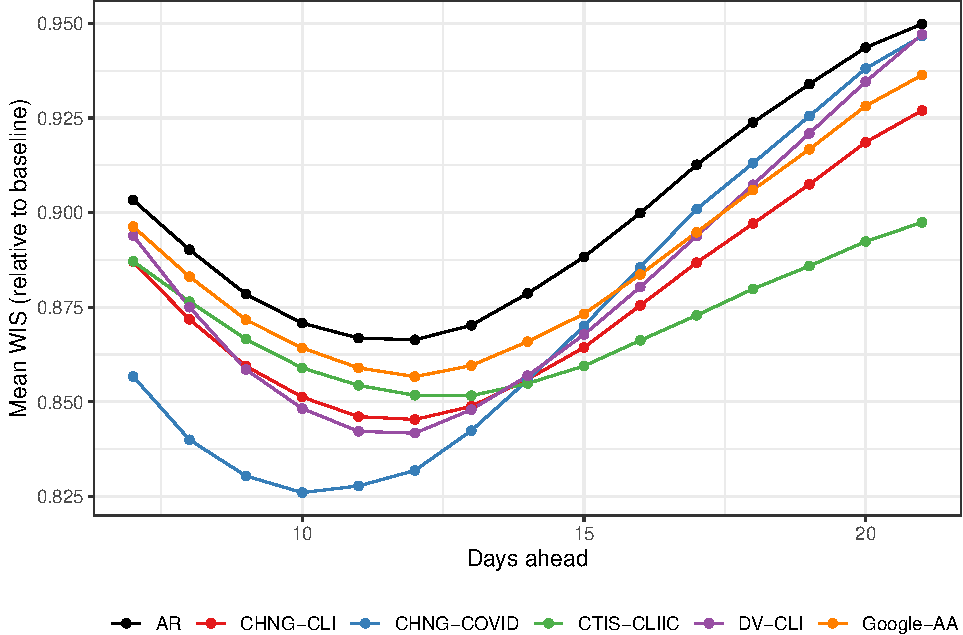
\includegraphics[width=\textwidth]{fig/fcast-finalized-1} 

}

\caption{Forecasting performance using finalized data. Compare to Figure 3 in the manuscript.}\label{fig:fcast-finalized}
\end{figure}

\clearpage

\begin{figure}

{\centering 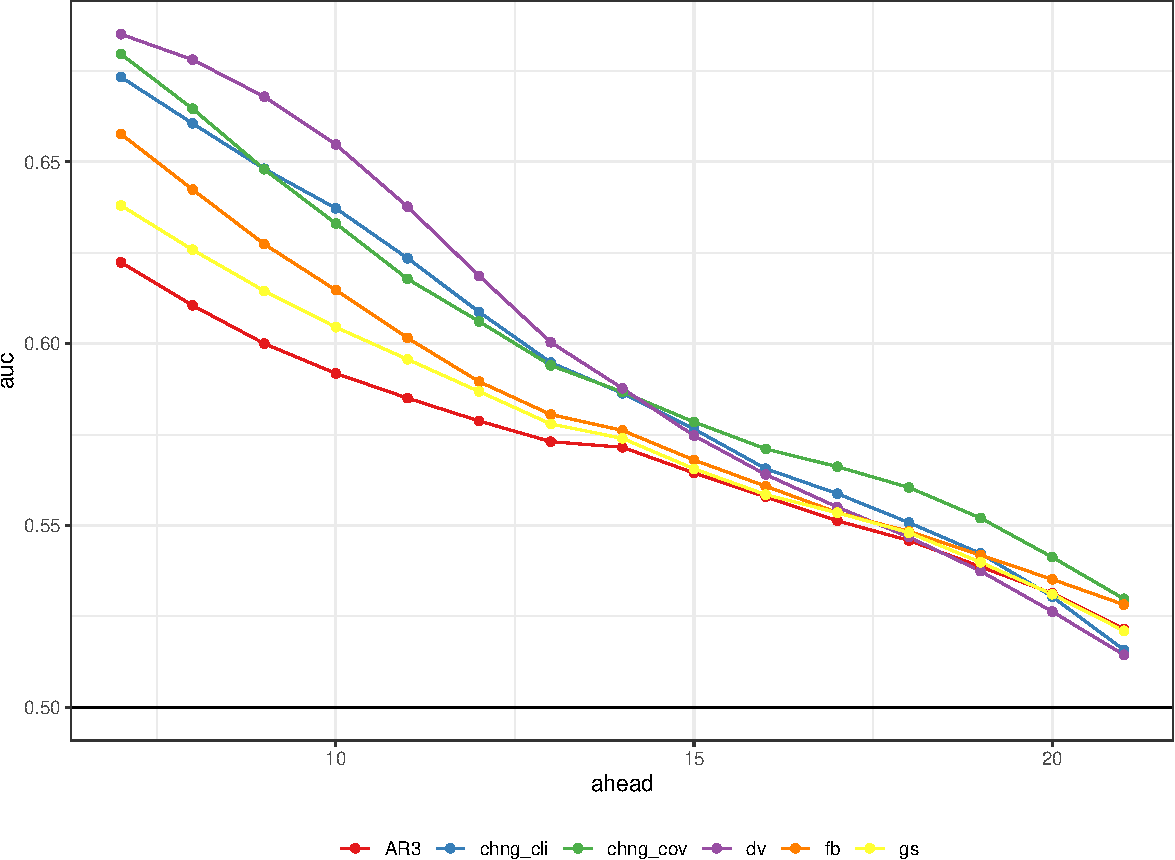
\includegraphics[width=\textwidth]{fig/hot-finalized-1} 

}

\caption{Hotspot prediction performance using finalized data. Compare to Figure 4 in the manuscript.}\label{fig:hot-finalized}
\end{figure}

\clearpage

\begin{figure}

{\centering 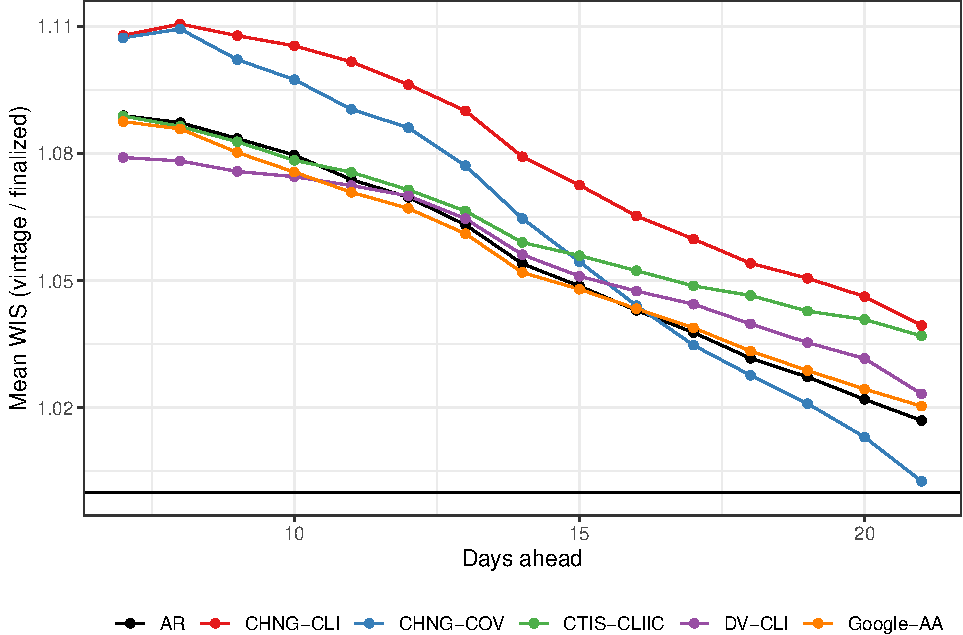
\includegraphics[width=\textwidth]{fig/fcast-honest-v-finalized-1} 

}

\caption{Relative forecast WIS with vintage compared to finalized data. Using finalized data leads to overly optimistic performance.}\label{fig:fcast-honest-v-finalized}
\end{figure}

\clearpage

\begin{figure}

{\centering 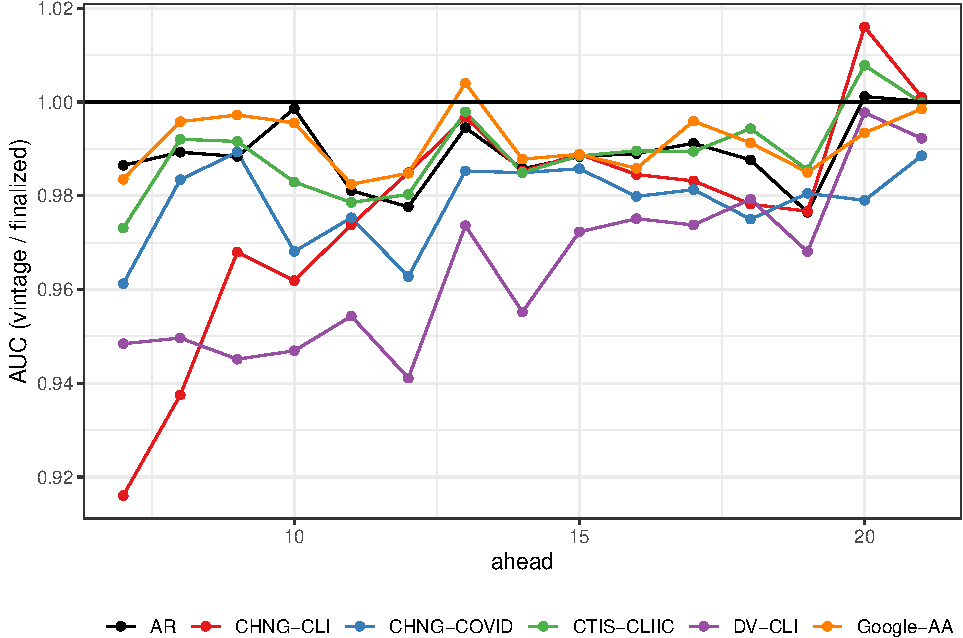
\includegraphics[width=\textwidth]{fig/hot-honest-v-finalized-1} 

}

\caption{Relative AUC with vintage compared to finalized data. Using finalized data leads to overly optimistic hotspot performance.}\label{fig:hot-honest-v-finalized}
\end{figure}

\clearpage

\begin{figure}

{\centering 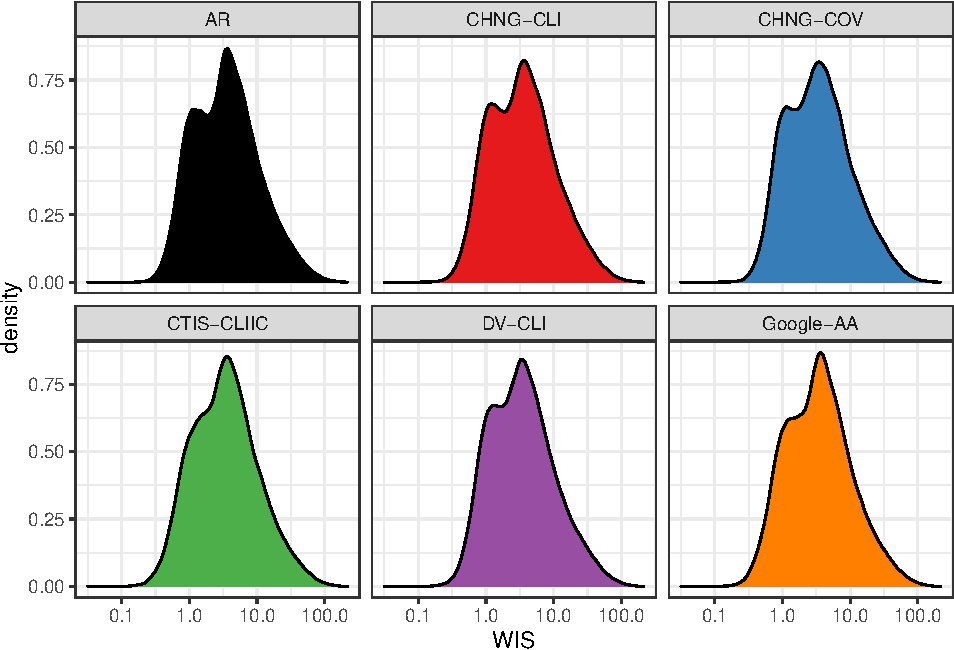
\includegraphics[width=\textwidth]{fig/wis-densities-1} 

}

\caption{Weighted interval score appears to more closely resemble a log-Gaussian distribution.}\label{fig:wis-densities}
\end{figure}

\clearpage

\begin{figure}

{\centering 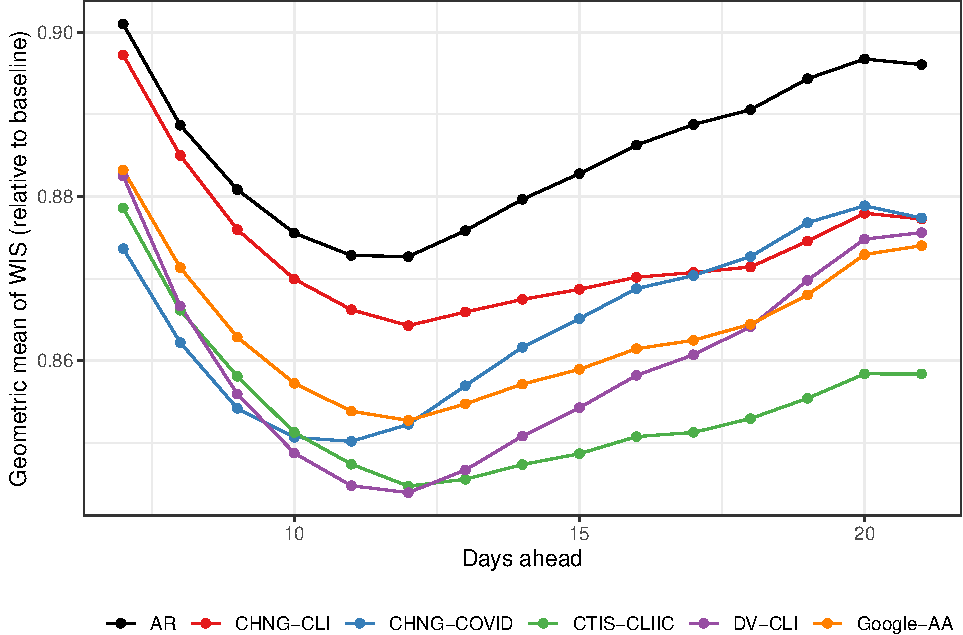
\includegraphics[width=\textwidth]{fig/fcast-adjusted-1} 

}

\caption{Relative forecast performance using vintage data and summarizing with the more robust geometric mean.}\label{fig:fcast-adjusted}
\end{figure}

\clearpage

\begin{figure}

{\centering 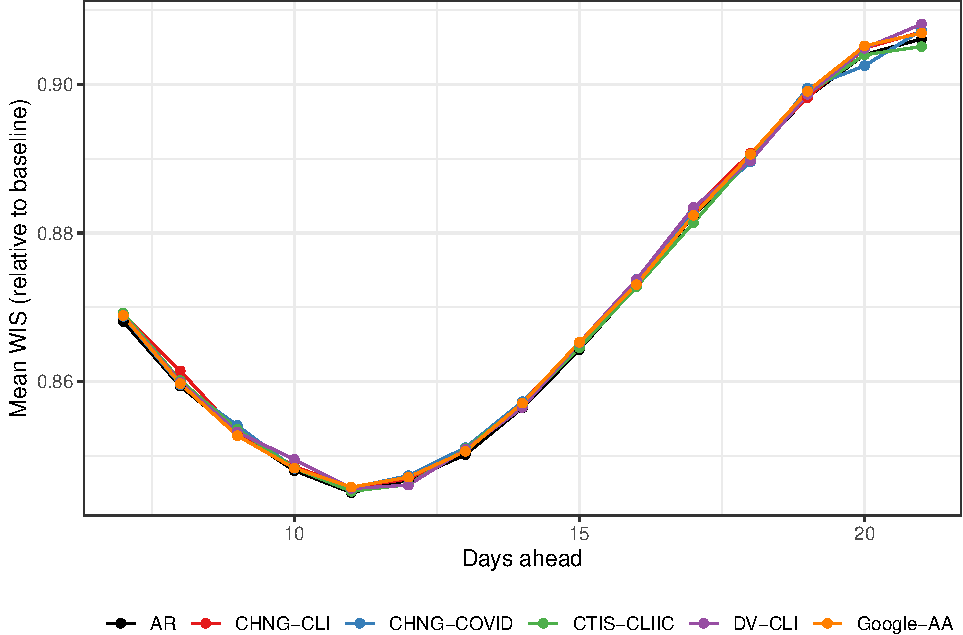
\includegraphics[width=\textwidth]{fig/fcast-booted-1} 

}

\caption{Forecast performance when indicators are replaced with samples from their empirical distribution. Performance is largely similar to the AR model.}\label{fig:fcast-booted}
\end{figure}

\clearpage

\begin{figure}

{\centering 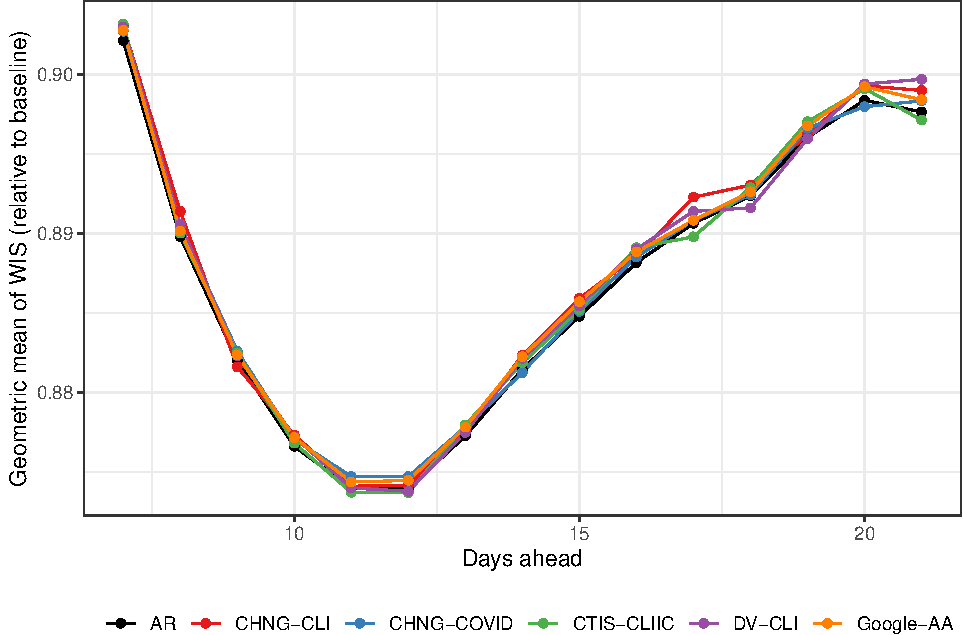
\includegraphics[width=\textwidth]{fig/fcast-booted-adjusted-1} 

}

\caption{Forecast performance as measured with the geometric mean when indicators are replaced with samples from their empirical distribution. Performance is largely similar to the AR model.}\label{fig:fcast-booted-adjusted}
\end{figure}

\clearpage

\begin{figure}

{\centering 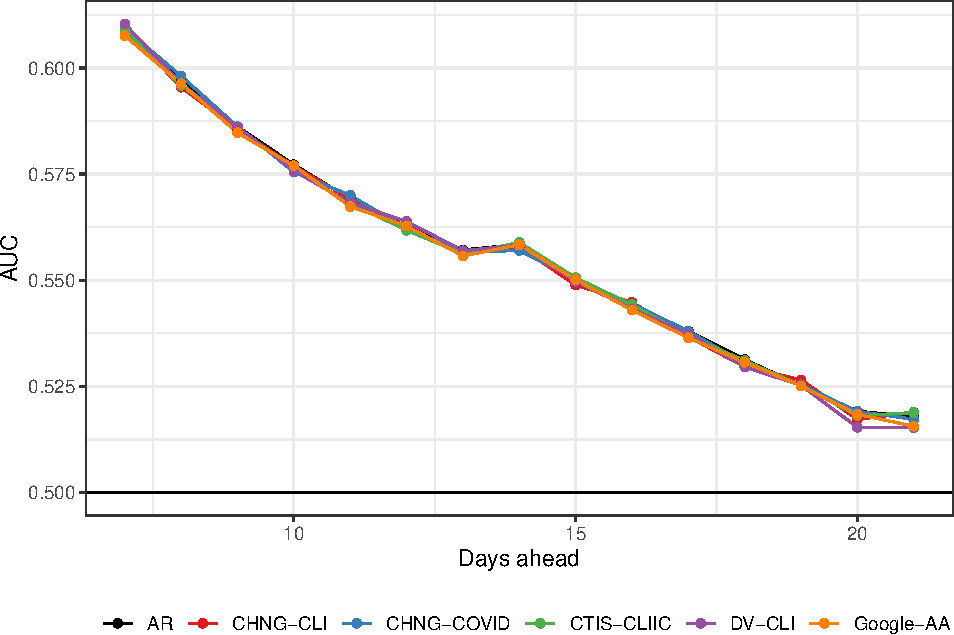
\includegraphics[width=\textwidth]{fig/hot-booted-1} 

}

\caption{Hotspot prediction performance when indicators are replaced with samples from their empirical distribution. Performance is largely similar to the AR model.}\label{fig:hot-booted}
\end{figure}

\clearpage

\begin{figure}

{\centering 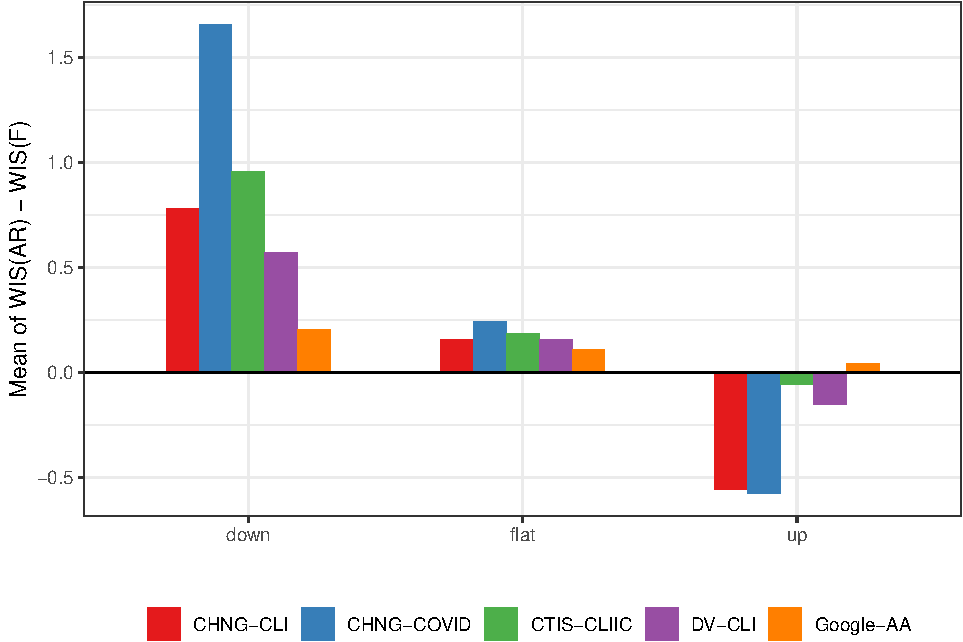
\includegraphics[width=\textwidth]{fig/upswing-summary-1} 

}

\caption{Average difference between the WIS of the AR model and the WIS of the other forecasters. The indicator-assisted forecasters do best during down and flat periods.}\label{fig:upswing-summary}
\end{figure}

\clearpage

\begin{figure}

{\centering 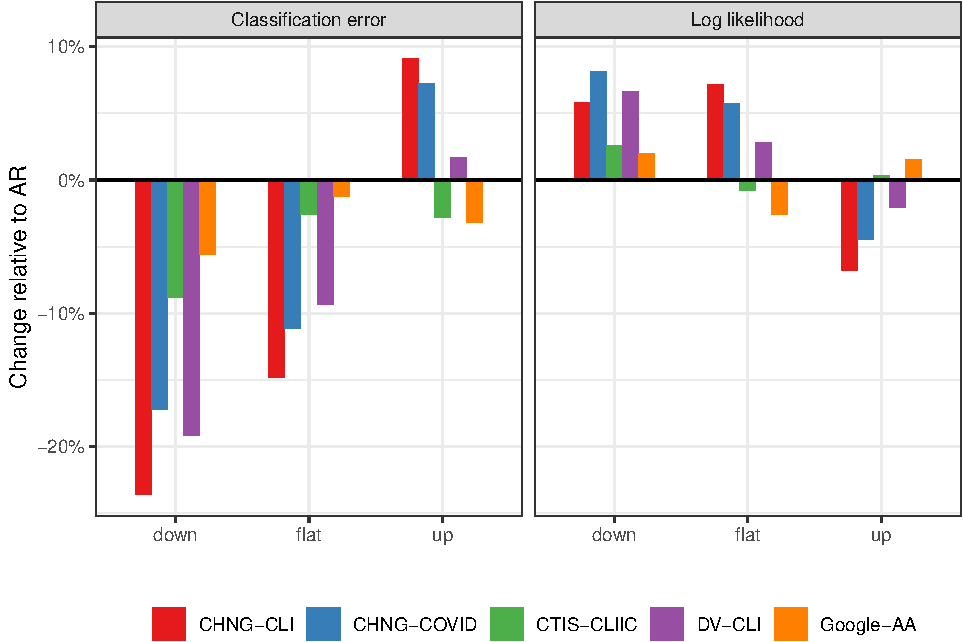
\includegraphics[width=\textwidth]{fig/hotspots-upswing-downswing-1} 

}

\caption{Classification and loglikelihood separated into periods of upswing, downswing, and flat cases. Like the analysis of the forecasting task in the main paper (see Figure 7), performance is better during down and flat periods.}\label{fig:hotspots-upswing-downswing}
\end{figure}

\clearpage

\begin{figure}

{\centering 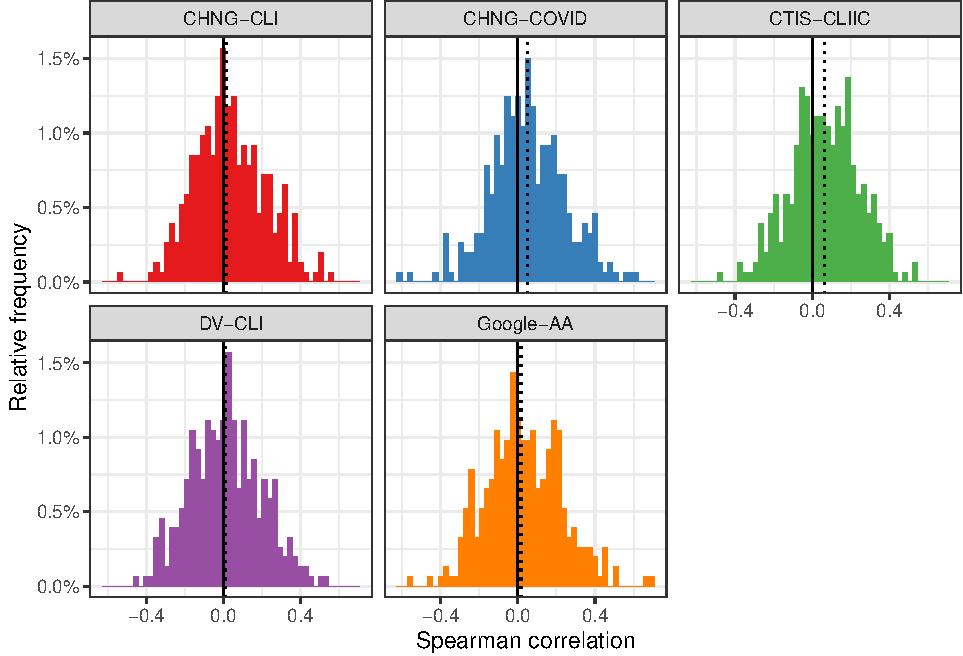
\includegraphics[width=\textwidth]{fig/cor-wis-ratio-1} 

}

\caption{Histograms of the Spearman correlation between the ratio of AR to AR WIS with the percent change in smoothed case rates relative to 7 days earlier.}\label{fig:cor-wis-ratio}
\end{figure}

\clearpage

\clearpage

\begin{figure}

{\centering 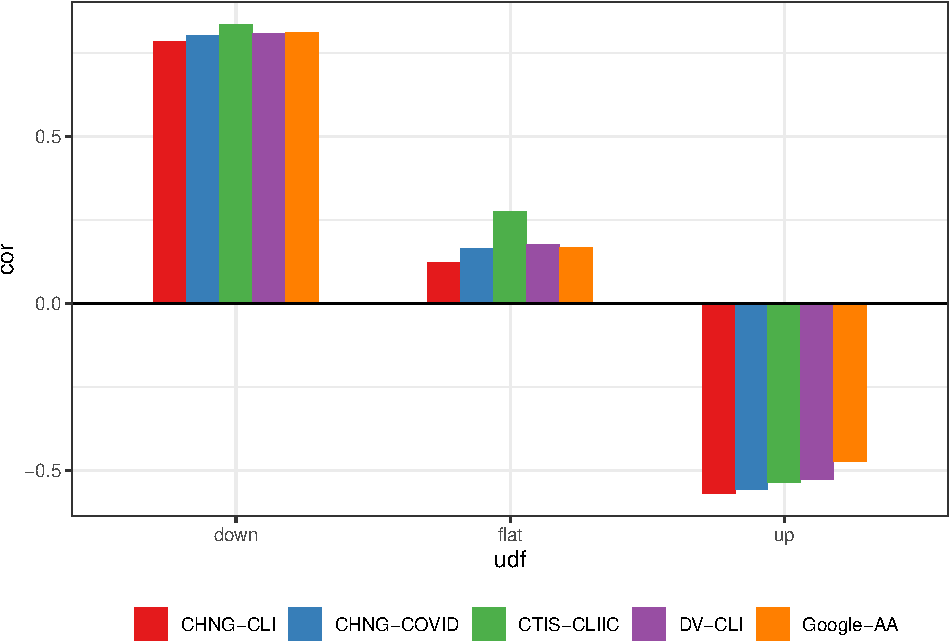
\includegraphics[width=\textwidth]{fig/upswing-corr-table-1} 

}

\caption{Correlation of the difference in WIS with the difference in median predictions for the AR model relative to the indicator-assisted forecaster. In down periods, improvements in forecast risk are highlycorrelated with lower median predictions. The opposite is true in up periods. This suggests, as one might expect that improved performance of the indicator-assisted model is attributable to being closer to the truth then the AR model. This conclusion is stronger in down periods then in up periods.}\label{fig:upswing-corr-table}
\end{figure}

\clearpage

\begin{figure}

{\centering 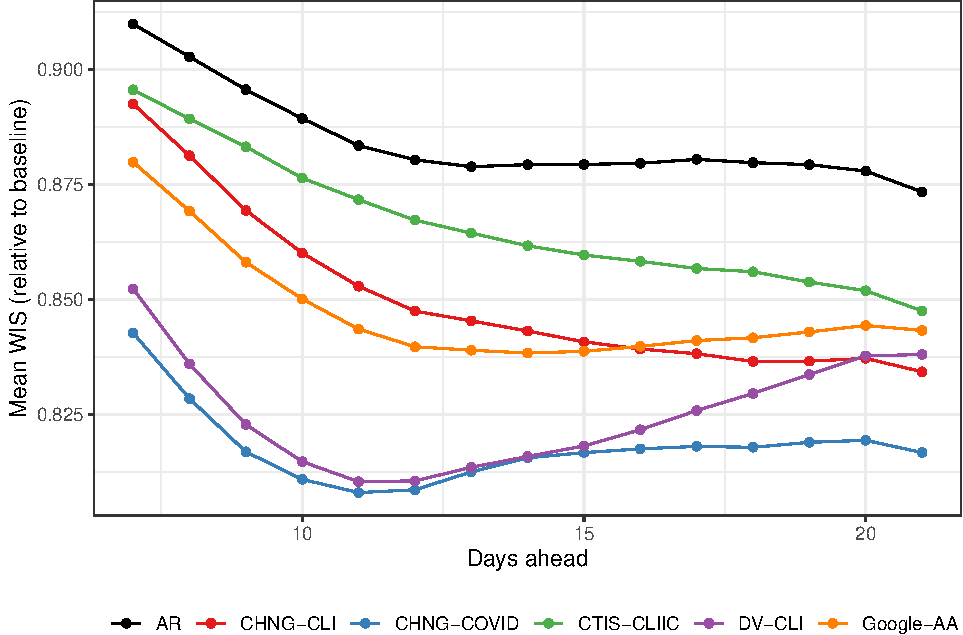
\includegraphics[width=\textwidth]{fig/fcast-alldates-1} 

}

\caption{Forecast performance over all periods. Performance largely improves for all forecasters with the inclusion of data in 2021.}\label{fig:fcast-alldates}
\end{figure}

\clearpage

\begin{figure}

{\centering 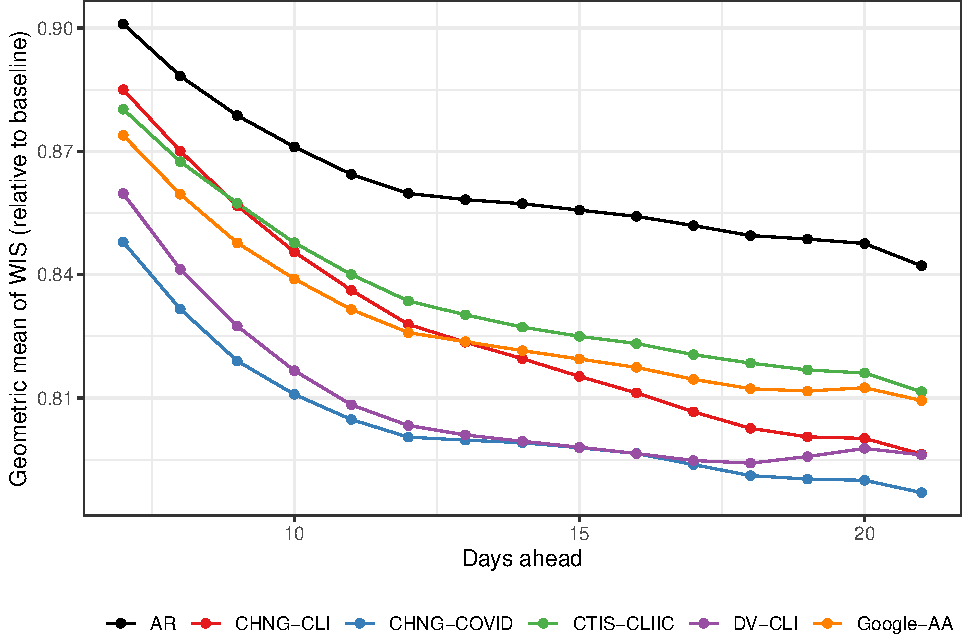
\includegraphics[width=\textwidth]{fig/fcast-alldates-adjusted-1} 

}

\caption{Forcast performance over all periods aggregaged with the geometric mean. Again, the inclusion of data in 2021 leads to improved performance.}\label{fig:fcast-alldates-adjusted}
\end{figure}

\clearpage

\begin{figure}

{\centering 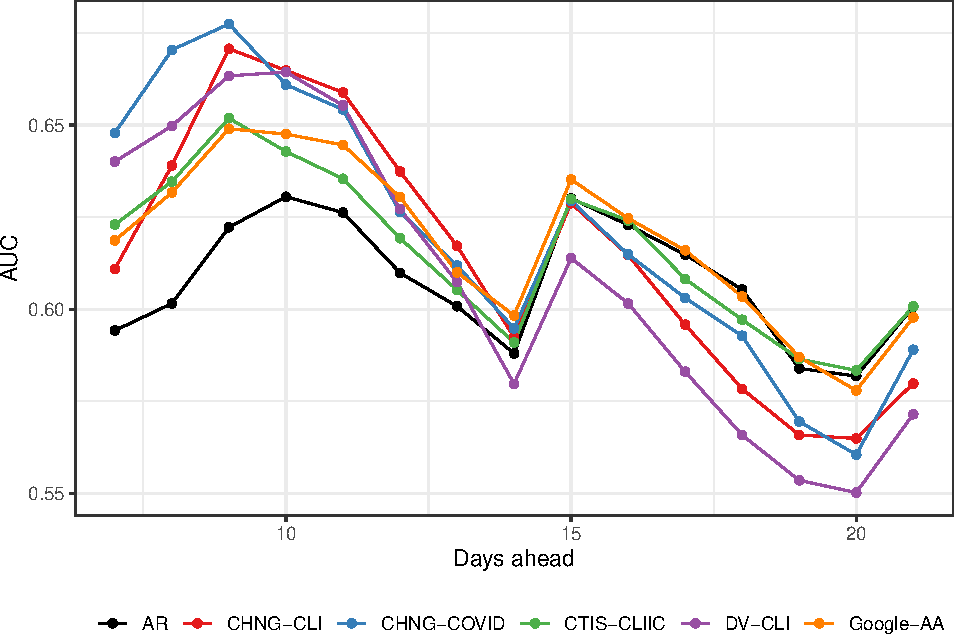
\includegraphics[width=\textwidth]{fig/hot-alldates-1} 

}

\caption{Area under the curve for hotspot predictions including data in 2021. Performance degrades relative to the period in 2020. However, there are far fewer hotspots during this period as case rates declined in much of the country.}\label{fig:hot-alldates}
\end{figure}

\clearpage

\FloatBarrier

\dataset{dataset_one.txt}{Type or paste legend here.}

\dataset{dataset_two.txt}{Type or paste legend here. Adding longer text to show what happens, to decide on alignment and/or indentations for multi-line or paragraph captions.}




\bibliography{../../common/covidcast.bib,pnas-materials/pnas-sample.bib}

\end{document}